\chapter{結果}
\section{ L1$_2$ クラスターおよび Small Cluster の導入}

\subsection{18層の slub モデルの計算結果}

18層の slub モデルの系全体のエネルギーの計算結果をまとめたグラフを図\ref{fig18} に示す. 18 層の計算では, 4 層の計算が収束しなかった. しかし, わずかではあるがエネルギー傾向が 5層から 7層で単調増加を示した. このままエネルギーが増加を示すと別の L1$_2$ クラスターから影響を受けている事を示唆する. 8層以降で増加が止まれば別の L1$_2$ クラスターからの影響ではなく Small Cluster が中距離で安定するという事が示唆される. しかし, それ以降の値が判明していなかったために, 8 層以降のエネルギー傾向が単調増加するかどうかが判明しなかった.

\begin{figure}[htbp]
	\begin{center}
		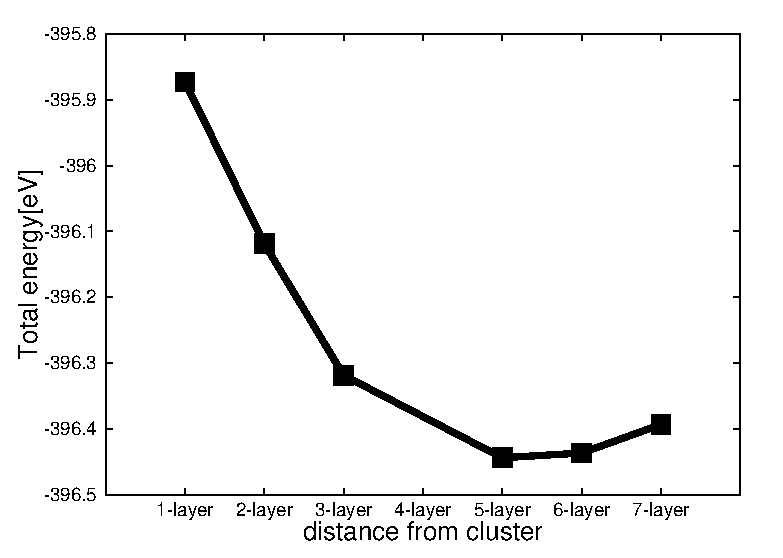
\includegraphics[width=100mm]{../result/small_cluster.eps}
		\caption{18層の slub モデルのエネルギー.}
		\label{fig18}
	\end{center}
\end{figure}

\subsection{C 層に Small Cluster を挿入した時のエネルギー}
クラスターから 1, 3, 5, 7, 9 層離れた層は C 層の原子配置であり, 図\ref{fig3.1} で示す. ここでは青丸は第 1 近接位置, 緑丸は第 2 近接位置, 黄丸は第 3 近接位置を表している. 表3.1 は C 層の第 1, 2, 3 近接距離に Small Cluster を挿入したモデルのエネルギーを表している.

\begin{figure}[htbp]
	\begin{center}
		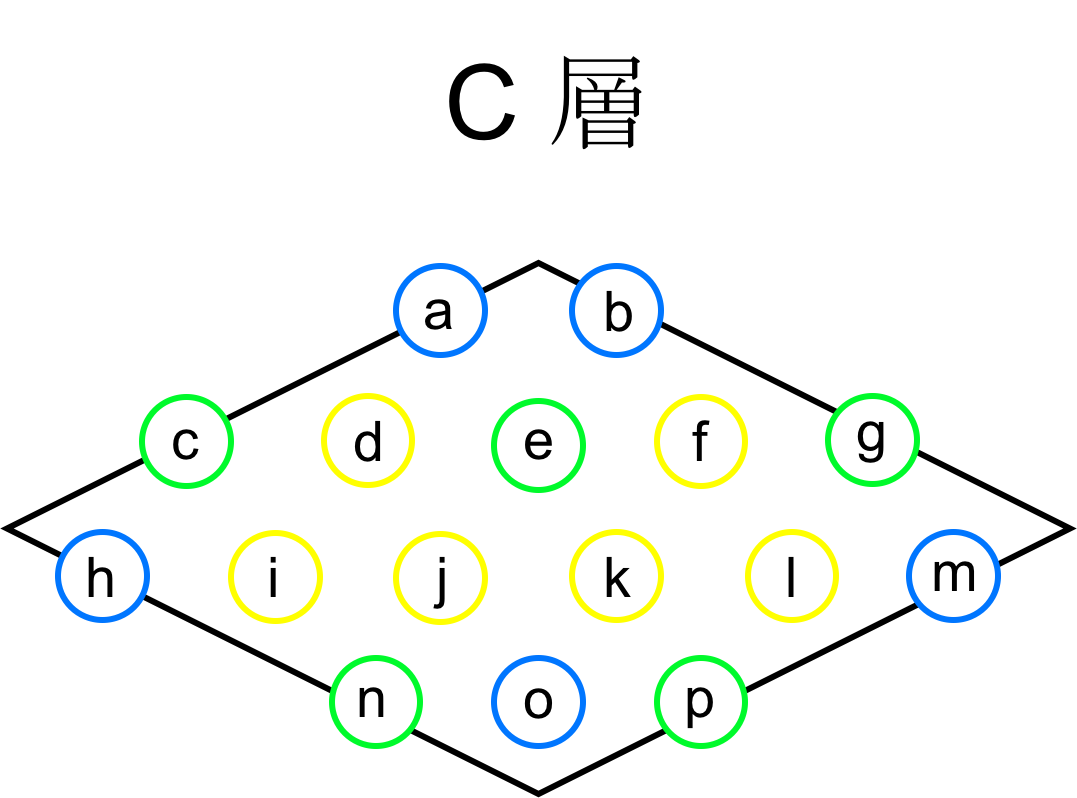
\includegraphics[width=90mm]{../method/Clayer.png}
		
\includegraphics[width=60mm]{../method/AClayer.png}
		\caption{C 層の第 0, 1, 2, 3 近接位置を表した模式図.}
		\label{fig3.1}
	\end{center}
\end{figure}

\begin{table}[H]
\caption{C 層の第 1, 2, 3 近接距離に Small Cluster を挿入したモデルのエネルギー [eV].}
  \begin{center}
    \begin{tabular}{|l|c|c|c|c|c|} \hline
         & 第 1 層 & 第 3 層 & 第 5 層 & 第 7 層 & 第 9 層\\ \hline
第 1 近接位置 & -506.773098 & -507.223404 & -507.339844 & -507.300403 & -507.274385\\
\hline
第 2 近接位置 & -506.872873 & -507.240530 & -507.340992 & -507.305620 & -507.279716\\
\hline
第 3 近接位置 & -506.975043 & -507.255849 & -507.342078 & -507.300835 & -507.273358\\
\hline
    \end{tabular}
  \end{center}
\end{table}


\subsection{A 層に Small Cluster を挿入した時のエネルギー}
クラスターから 2, 4, 6, 8, 10 層離れた層は A 層の原子配置であり, 図\ref{fig3.2} で示す. ここでは赤丸は第 0 近接位置, 青丸は第 1 近接位置, 緑丸は第 2 近接位置, 黄丸は第 3 近接位置を表している. 表3.2 は A 層の第 0, 1, 2, 3 近接距離に Small Cluster を挿入したモデルのエネルギーを表している.

\begin{figure}[htbp]
	\begin{center}
		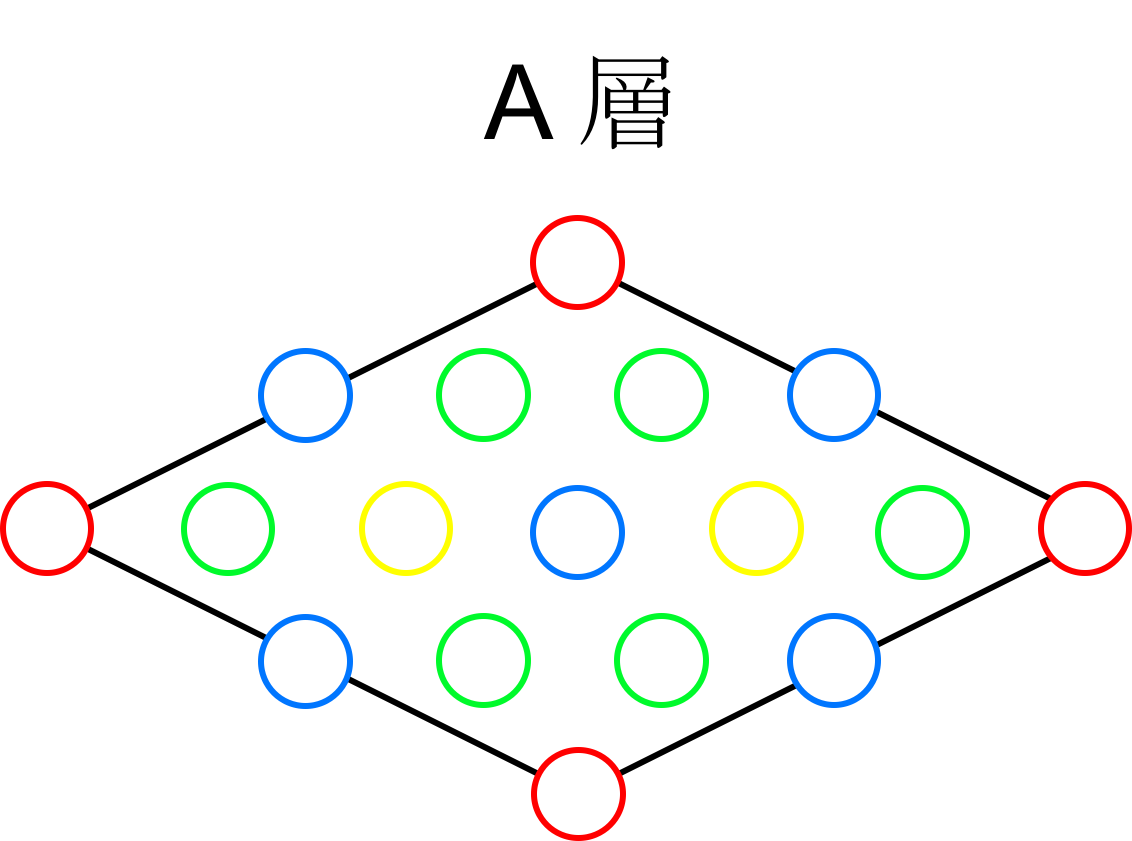
\includegraphics[width=90mm]{../method/Alayer.png}
		
\includegraphics[width=60mm]{../method/AClayer.png}
		\caption{A 層の第 0, 1, 2, 3 近接位置を表した模式図.}
		\label{fig3.2}
	\end{center}
\end{figure}

\begin{table}[H]
\caption{A 層の第 0, 1, 2, 3 近接距離に Small Cluster を挿入したモデルのエネルギー [eV].}
  \begin{center}
    \begin{tabular}{|l|c|c|c|c|c|} \hline
         & 第 2 層 & 第 4 層 & 第 6 層 & 第 8 層 & 第 10 層\\ \hline
第 0 近接位置 & -507.041788 & -507.340218 & -507.324580 & -507.264994 & -507.274057\\
\hline
第 1 近接位置 & -507.095924 & -507.313473 & -507.327796 & -507.279462 & -507.274801\\
\hline
第 2 近接位置 & -507.117741 & -507.307283 & -507.334387 & -507.283037 & -507.272749\\
\hline
第 3 近接位置 & -507.152164 & -507.348526 & -507.336189 & -507.273986 & -507.275103\\
\hline
    \end{tabular}
  \end{center}
\end{table}

図\ref{fig3.3} は表 3.1 と表 3.2 のエネルギー値をグラフにまとめたものである. 赤点は第 0 近接位置, 青点は第 1 近接位置, 緑点は第 2 近接位置, 黄点は第 3 近接位置のエネルギーである.

\begin{figure}[htbp]
	\begin{center}
		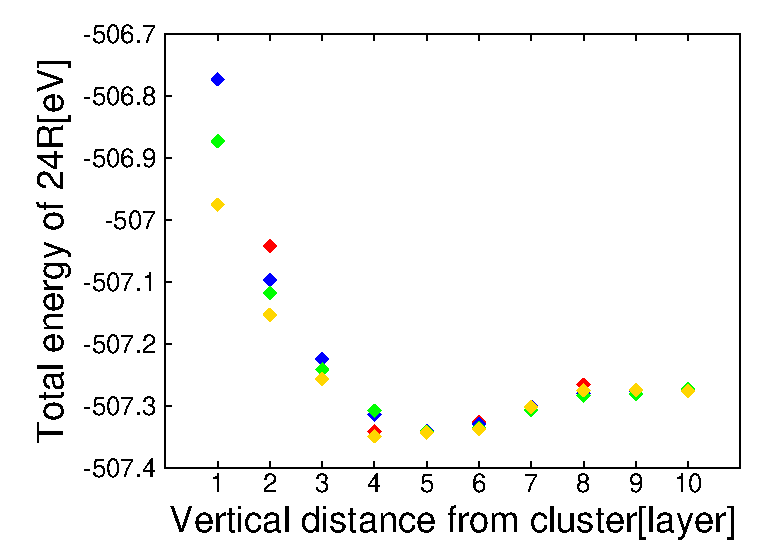
\includegraphics[width=90mm]{../result/small_cluster_Alld_color.eps}
		\caption{各層のエネルギーをまとめたグラフ.}
		\label{fig3.3}
	\end{center}
\end{figure}


\section{ Small Cluster および 空孔の導入}
1層12原子として, 6層の純粋な hcp-Mg 結晶がもつ系全体のエネルギーは -249.815039 eV である. 空孔を含む 6 層の Mg 結晶の系全体のエネルギーは -247.517691 eV である. これらの計算結果から空孔の形成エネルギーを算出した. 空孔の形成エネルギーの計算方法は以下の通りである.

\begin{enumerate}
 \item 純粋な Mg 結晶の結果から, hcp-Mg 1個が持つエネルギーを算出.\\ -249.815039/162;\\
-1.542068142
 \item 1 個のエネルギーから本来の Mg 161 個が持つエネルギーを算出.\\
-1.542068142*161;\\
-248.2729709
 \item 2 項目で得られた値とincludeの値の差を計算.\\
-248.2729709-(-247.517691);\\
-0.7552799
\end{enumerate}
これがこれが空孔の形成エネルギーである.


図\ref{fig2.4} のモデルにおいて, 空孔を挿入したモデルのエネルギーを表 3.3に示す.

\begin{table}[htb]
\caption{空孔を挿入した時のエネルギー.}
  \begin{center}
    \begin{tabular}{|l|c|c|c|c|c|} \hline
 挿入位置 & エネルギー [eV] \\ \hline
   (a) & -268.452640\\
\hline
   (b) & -267.932411\\
\hline
   (c) & -268.496561\\
\hline
    \end{tabular}
  \end{center}
\end{table}
